\documentclass{beamer}
\mode<presentation>
{
  \usetheme{Luebeck}
  \usecolortheme{beaver}
  \usefonttheme{default}
  \setbeamertemplate{navigation symbols}{}
  \setbeamertemplate{caption}[numbered]
  \setbeamertemplate{theorems}[numbered]% Number theorem-related structures
}
\usepackage{hyperref}
% include.tex

% \newcommand{\expit}[1]{\text{expit} #1}
% \newcommand{\logit}[1]{\text{logit} #1}

\def \R {{\mathbb{R}}}
\def \vbeta {{\boldsymbol \beta}}
\def \vnu {{\bf \nu}}
\def \vy {{\bf y}}
\def \vx {{\bf x}}
\def \vu {{\bf u}}
\def \vr {{\bf r}}
\def \vp {{\bf p}}
\def\vectorfontone{\bf}
\def\vone{{\bf 1}}
\def\vzero{{\bf 0}}
\def \vmu {{\boldsymbol \mu}}
\def \vnu {{\bf \nu}}
\def \vmuqbeta {{\vmu_{q(\vbeta)}}}
\def \vmubeta {{\vmu_{\vbeta}}}
\def \Sigmaqbeta {{\Sigma_{q(\vbeta)}}}
\def \Sigmabeta {{\Sigma_{\vbeta}}}
\def \va {{\bf a}}
\def \vtheta {{\bf \theta}}
\def \mX {{\bf X}}
\def \mZ {{\bf Z}}
\def \mR {{\bf R}}
\def \mC {{\bf C}}
\def \mI {{\bf I}}
\def \mLambda {{\boldsymbol \Lambda}}
\def \mSigma {{\boldsymbol \Sigma}}
\def \B {{\text{B}}}

\def\ds{{\displaystyle}}

\def\diag{{\mbox{diag}}}
\def\bbE{\mathbb{E}}

\title{Why is my code so slow?}
\author{Mark Greenaway}

%\begin{frame}
%Abstract

%Why is my code so slow?

%Many of us have been frustrated by running a program to perform a numerical
%experiment or a calculation and having it take a long time. In this talk, I
%will give a brief history of computers as it relates to performance, touching
%on cache hierarchy, the end of Moore's Law, multicore/GPUs and distributed
%computing. I will explain the latencies within a modern computer system, and
%the implications of this. I'll briefly provide a methodology for measuring and
%optimising the speed of programs.  Finally, I'll provide a glimpse into the
%future of computing and why it's going to be better than the present/past.

%This talk is supposed to be accessible to everyone, and as such, there will be
%no assumed knowledge.

%Mark Greenaway did a PhD supervised by A/Prof John Ormerod in computational
%statistics. He enjoys High Performance Computing, programming in statically
%typed languages, drinking too much coffee and listening to heavy metal music.
%Preferably all at the same time.
%\end{frame}

\begin{document}
\begin{frame}
	\maketitle
\end{frame}

\begin{frame}{Who am I?}
	\begin{itemize}
		\item Mark Greenaway, kind of old
		\item Bachelor of Computer Science, UWS, 1995--1997
		\item I have a UNIX/Linux upbringing, having used Linux since 1993
		\item Over a decade of software engineering experience. I now lead a small team at the Commonwealth Bank, working on microservices for security
		\item
			\begin{itemize}
				\item Bachelor of Pure Mathematics and Statistics (Honours I), USyd, 2006--2009
				\item Masters of Biostatistics
				\item PhD in Computational Statistics (accepted with minor revisions), working with A/Prof John Ormerod
			\end{itemize}
	\end{itemize}
	I'm very opinionated, but I will attempt to present facts and let you decide for yourselves. If you want to know my opinion, read my Twitter at @certifiedwaif or ask me
\end{frame}

\begin{frame}{Why do mathematicians or statisticians care about computers at all?}
	\begin{itemize}
		\item I'm a computational statistician, so that informs my perspective
		\item The Bayesian perspective: Bayes' Theorem
			$$p(\vtheta|\vy, \mX) \propto \int p(\vy|\vtheta, \mX) p(\vtheta) d \vtheta$$ \\
			Many of the resulting integrals are analytically intractable and must be evaluated numerically
			\note{Bayesians know how to solve any statistical estimation problem, by turning your model specification into an integral we can't do}
		\item Relieves us of computational burden - we can't do many problems of practical interest with paper and pen
		\item{Numerical Recipes} -- All numerical problems seem to break down to function evaluation or linear algebra. If you're an applied mathematician, maybe differential equation solvers as well? 
	\end{itemize}
\end{frame}

\begin{frame}{Why does the speed of your code matter?}
	\begin{itemize}
		\item If your programs complete in seconds, or minutes, maybe they're fast enough
	already.  If they start to take minutes or hours, maybe not
	\note{and you're waiting for the
	results before you can do anything else, the speed of your code dictates the
	speed of your research.  For some areas of research, like computational fluid
dynamics, bioinformatics or others, computational speed becomes the limiting factor}
	\item An order of magnitude isn't just more of the same.  New things become possible
		\note{for example, the difference between powering a land vehicle and being able to get and keep it airborne is about a factor of ten New things become possible when you have access to this much computing power -- different approaches. Bigger problems, more dimensions, $p >> n$}
	\item \emph{Example: Bayesian Model Averaging} -- The amount of computation is extreme, and runtimes of days, weeks or months are not unheard of. It has been unfavorably compared to cryptocurrency mining \note{which contributes to climate change CO_2}
\item If a primary output of your research is software, then you're likely to be
	judged on how quickly that software runs
	\note{In my field, every paper includes
	both numerical results and runtimes. If you can produce an equally numerically
	accurate result in less runtime, your software is better and you can publish a
paper on that.}
	\item If you're writing software for other people to use, if it takes too long, they just won't use it
	\note{I worked as an applied statistician for years. If a model took more than a few minutes to run, I'd usually just give up and try something else. The reason I ended up back here is that I ran a model which took ten minutes to run and then failed to converge (!). This \emph{really} pissed me off.}
	\end{itemize}
\end{frame}

\begin{frame}{Caveat: When does the speed of your code \emph{not} matter?}
	\begin{itemize}
		\item Speed can mean different things in different contexts. Maybe what matters isn't
	how fast the computer runs your code, but how quickly you can do your analysis
	and move on to something else. \texttt{R}/\texttt{tidyverse} optimises for this

\item What really matters is the speed of your research \note{Is your thesis finished yet? Have you written that paper? How's that grant coming along?}
	\note{You need to balance the
	amount of time spent on getting software to run faster against the amount of
time actually saved by having it run for less time.}
	\item Optimising code to run faster should not trump every other research goal
	\item Maybe your time is better spent writing a paper or a grant, making a
plot look better, or working on a thesis chapter? It's your call
\end{itemize}
\end{frame}

\begin{frame}{What do computers actually do? - CPU}
	A computer consists of a few major components
	\begin{itemize}
		\item The Central Processing Unit (CPU) does a few things
			\begin{enumerate}
				\item arithmetic/logic
				\item conditional and unconditional branching
				\item reading/writing memory
				\item input/output to devices like keyboards, display adapters, disks, network interfaces, \ldots
		\end{enumerate}
		They do this by running very simple instructions, like \texttt{mov \%eax, 10} which moves the value $10$ into the first register on an Intel CPU.
	\item A CPU runs an instruction in between one and a few clock cycles, but it runs \emph{billions} of these instructions per second
\end{itemize}
\end{frame}

\begin{frame}{What do computers actually do? - Memory}
	\begin{itemize}
		\item CPUs have built in memory locations, called registers. The CPU's instructions
			can operate on these, or on memory on some architectures. Because the registers are on the chip, they're super fast
		\item For working with more data than can fit in the registers, We use memory off the CPU called RAM to load and store our data. It's cheaper, but slower to read and write
		\item That memory only lasts as long as the computer is on, so we load and save our data more permanently on disks. Those are cheaper, but slower still
		\item Computers can also communicate with each other over a network, to the Local
			Area Network or Internet. Which is great, but \emph{really} slow
	\end{itemize}
\end{frame}

% TODO(Mark) You need a picture
% Diagram: https://stackoverflow.com/questions/28815848/does-each-core-has-its-own-private-set-of-registers
\begin{frame}{A diagram of a CPU -- Intel core i7 Nehalem microarchitecture}
	\begin{figure}
		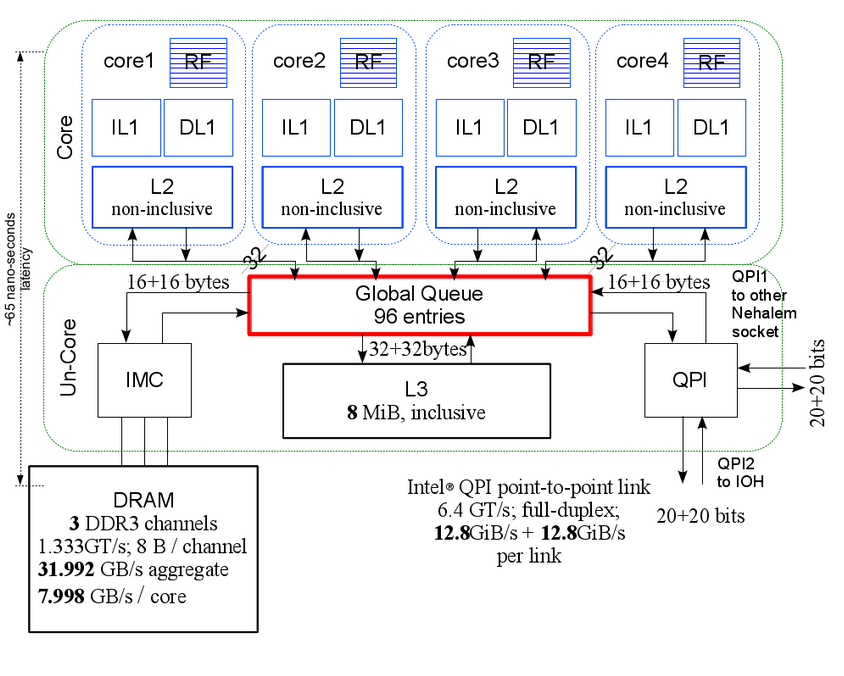
\includegraphics[scale=0.5]{Intel_core_i7.png}
	\end{figure}
\end{frame}

\begin{frame}{What do computers actually do? - Software}
	\begin{itemize}
		\item The Operating System kernel manages computer resources like scheduling when
			user programs run, which memory each program uses and access to the hardware
		\item User level programs ask the kernel to do things for
			them, like allocate memory, start a process, read a file or send data over the
			network to another computer
	\end{itemize}
\end{frame}

\begin{frame}{Programming languages}
	\begin{itemize}	
		\item Computers run assembly language. Computers were originally programmed in assembly or machine code, but this took a long time, and was tedious and error prone\note{show an example, the dot\_product}
		\item To allow programmers to be more productive, higher level languages like Fortran and C were invented
\item  And then even more high level ones, like R and Python. Python and R are ``glue'' languages that make calling C and Fortran easy, should you need to
		\item There are two major ways that code gets converted to instructions for computers to run: \emph{compilers} and \emph{interpreters}
			\begin{itemize}
				\item{compiler} Convert an entire program into assembly language at once
				\item{interpreter} Interpret a statement, then execute it
			\end{itemize}
	\end{itemize}
\end{frame}

\begin{frame}{Differences between programming languages}
	\begin{itemize}	
		\item C and Fortran require you to manually allocate and deallocate memory, and declare types \note{Unsafe
	memory access, leading to the possibility of segmentation faults where
you attempt to access a piece of memory that's not yours. You need to tell them what type your variables are so it knows how much memory they need, and how that memory is laid out}
		\item R and Python use reference-counting garbage collection to manage memory for you, and are safe and dynamically typed \note{They manage the layout and allocation/deallocation of memory for you}
\item There is a difference in speed: Rust versus R example https://rustr.org/
\item Array languages like R and Matlab get us out of trouble most of the time, and save us from writing as many loops ourselves. This is why people say ``\texttt{for} loops are slow''
	\note{BLAS executes your for loops for you in highly optimised Fortran or C, where they're fast}
	\end{itemize}
\end{frame}

\begin{frame}{Brief history of computer hardware}
	\begin{itemize}
 \item 1970s -- 8-bit, clock speeds measure in kilohertz, in the 8-bit 6502 era memory was fast enough to keep up with the CPU. Most of the programming languages that we use today use a flat memory model which dates from this time, and assumes that all memory takes the same amount of time to access. This has not been true since at least 1985 for most of us
\item For a while, Moore's Law continues -- Every year, the clock speed doubles \\
	Clock speeds keep increasing, but memory and disk does \emph{not} kept pace \\
	\emph{Solution:} Cache/Memory hierarchy! RAID disk arrays!

\item	2010s -- You can buy a 4 GHz CPU now, but are we at the end of Moore's Law? \textbf{YES!}\\
	\note{About the beginning of the 2010s, clock speeds stopped increasing. Reference Sophie Wilson's talk on the Future of Microprocessors.}
	\emph{Solutions:} Vector units! More cores! GPUs! Distributed computing! Solid State Drives become available, which are much faster than hard disks
	\end{itemize}
\end{frame}

% Credit: https://gist.github.com/jboner/2841832
\begin{frame}{Latency}
	Everything you do on a computer takes time. Some things are fast, and some of them are
	comparatively very slow.
	{
	\tiny
			\begin{tabular}{lllll}
Task & ns & us & ms & Note \\
\hline
L1 cache reference                &          0.5 ns &&& \\
Branch mispredict                 &          5   ns &&& \\
L2 cache reference                &          7   ns &&                   &14x L1 cache \\
Mutex lock/unlock                 &         25   ns &&& \\
Main memory reference             &        100   ns &&                   &20x L2 cache, 200x L1 cache \\
Compress 1K bytes with Zippy      &      3,000   ns &      3 us&& \\
Send 1K bytes over 1 Gbps network &     10,000   ns &     10 us&& \\
Read 4K randomly from SSD*        &    150,000   ns &    150 us&         &~1GB/sec SSD \\
Read 1 MB sequentially from memory&    250,000   ns &    250 us&& \\
Round trip within same datacenter &    500,000   ns &    500 us&& \\
Read 1 MB sequentially from SSD*  &  1,000,000   ns &  1,000 us  & 1 ms &~1GB/sec SSD, 4X memory \\
Disk seek                         & 10,000,000   ns & 10,000 us  &10 ms &20x datacenter roundtrip \\
Read 1 MB sequentially from disk  & 20,000,000   ns & 20,000 us  &20 ms &80x memory, 20X SSD \\
Send packet CA \to Netherlands \to CA&150,000,000 ns&150,000 us&150 ms
\hline
			\end{tabular}
		}
			What you should focus on here aren't the specific \emph{numbers}, but the difference in
	\emph{magnitude}.
\end{frame}

% Credit: https://twitter.com/DynamicWebPaige/status/1044443943679668224/photo/1
\begin{frame}{Latency -- graphically}
	\begin{figure}
		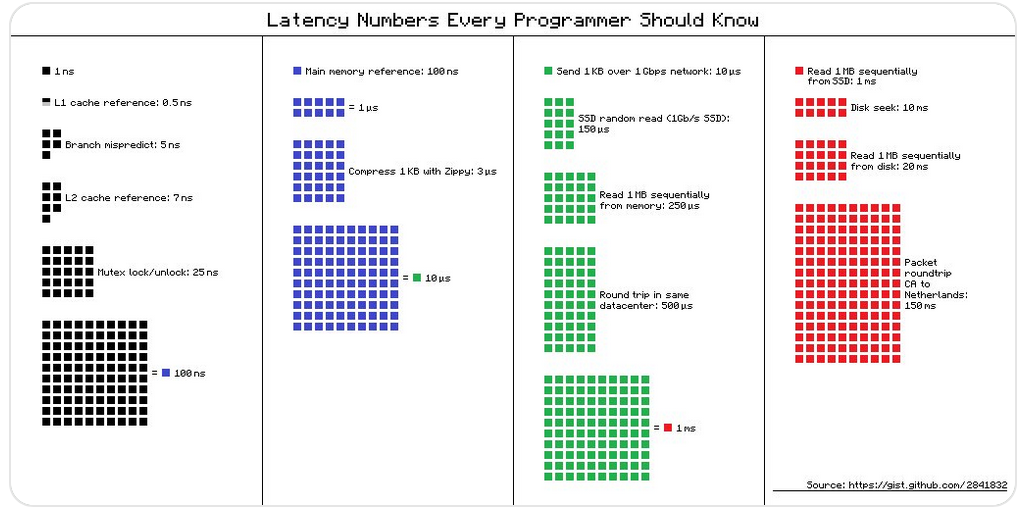
\includegraphics[scale=0.60]{Latency_graphically.png}
	\end{figure}
\end{frame}

\begin{frame}{What should we do to speed things up?}
	\begin{itemize}
		\item Make sure your program is correct first
		\item Measure where the time is spent with a profiler. Don't guess!
		\item Change from a higher strength operation to a lower strength operation that does the same thing where the bottleneck is. For example, in R, change a \texttt{for} loop to a vector operation, or use a lower level language
		\item Check correctness and measure the performance again. If your program is faster, congratulations, you're winning
		\item If not, back out the change and try again
		\item Repeat until your program is fast enough
	\end{itemize}

\end{frame}

\begin{frame}{Parallel Programming}
	\begin{itemize}
		\item Processes and Threads -- your operating system presents two major abstractions for programs to run in, threads and processes
		\item Cores have their own registers and L1 and L2 caches. L3 cache is shared amongst all cores. Memory and memory bandwidth is also shared
		\item Threads within a process have shared memory whereas processes each have their own memory
		\item For example, OpenMP is shared memory concurrency while \texttt{mclapply}/\texttt{future} is multi-process
		\item Shared memory concurrency opens up the possibility of \emph{race conditions}. Code that does not have any race conditions is said to be \emph{thread-safe}
		\item Languages which use reference-counting garbage collection are a textbook example of a race condition. They are not even \emph{remotely} thread-safe -- examples are R and Python
	\end{itemize}
\end{frame}

\begin{frame}{Parallel programming for Linux/Mac OS X and Windows}
	\begin{itemize}
		\item Linux and Mac OS X use very similiar UNIX kernels -- System V and BSD respectively. Programmers greatly prefer this
		\item Windows uses its own kernel, developed entirely by Microsoft
		\item Windows and UNIX have different operating system kernels, with different APIs. Windows presents a different threading API than UNIX
		\item \texttt{R} for Windows is a port of a UNIX program to Windows, but it is not a complete port.
		\item R for Windows is using the UNIX threading and multiprocess APIs through a compatibility library provided by a port of \texttt{gcc} to Windows, to try to make Windows look like UNIX to R.  But it doesn't work very well, which is why parallel programming in R doesn't work well on Windows
			\note{In fact, R for Windows doesn't work very well. Just ask the R for Windows maintainer, Jeroen Ooms @opencpu.  I'll quite happily tell you this}
	\end{itemize}
\end{frame}

\begin{frame}{What's coming?}
	\begin{itemize}
		\item Better hardware -- higher core counts, GPUs with more cores
			\begin{itemize}
				\item You can get a Power9 system with 144 cores for \$3,500, delivered.  You could get two of them -- 288 cores. And Power10 is due soon.
				\item Intel is releasing CPUs with higher core counts.
				\item NVidia is releasing GPUs with more and more cores.
			\end{itemize}

		\item Better languages -- allowing you to use this hardware more easily
			\begin{itemize}
				\item Better compilers
				\item Better libraries e.g. TensorFlow
				\item Just-In-Time compilers/interpilers
			\end{itemize}
	\end{itemize}
\end{frame}

\begin{frame}{What should I do?}
	\begin{itemize}
\item You can't buy a single core computer any more, so you should at least be aware of multithreaded programming
\item Any increases in computational speed are going to come from higher thread counts, GPUs or distributed computing
\item There is nothing else on the horizon, because physical limits are being reached. If
	we ran our CPUs any faster, \emph{they'd melt} \note{Reference Sophie Wilson's talk again}
\item If you're doing all of your computing on your laptop, you're \emph{really}
	missing out. You should at least know how to use servers
\item I assembled a small HPC cluster for \$100 per node. Ask me how! Computers have become very cheap
\item We have lots of research servers, and HPC have thousands of computers. Make good use of
	them.
\item The cloud is someone else's computer, they'll rent by the hour. Computing is now a commodity.
	\end{itemize}
\end{frame}

\end{document}
